\documentclass[11pt,a4paper]{article}
\usepackage[margin=2cm]{geometry}
\usepackage[T1]{fontenc}
\usepackage[default]{sourcesanspro}
\usepackage[scale=0.86]{sourcecodepro}
\usepackage{microtype}
\usepackage{setspace}
\usepackage{xcolor}
\usepackage[most]{tcolorbox}
\usepackage{booktabs}
\usepackage{longtable}
\usepackage{array}
\usepackage{graphicx}
\usepackage{caption}
\usepackage{enumitem}
\usepackage{titlesec}
\PassOptionsToPackage{obeyspaces,spaces}{url}
\usepackage{xurl}
\usepackage[hidelinks]{hyperref}
\usepackage{tikz}
\usetikzlibrary{positioning,arrows.meta}
\tikzset{box/.style={draw=accent,fill=accent!7,rounded corners=2pt,align=center,inner sep=2.5pt,minimum height=9mm,text width=#1},box/.default=19mm,
  soft/.style={draw=black!35,fill=black!4,rounded corners=2pt,align=center,inner sep=2.5pt,minimum height=9mm,text width=#1},soft/.default=19mm,
  arr/.style={-{Stealth[length=1.6mm]},accent,thick}}

\definecolor{accent}{HTML}{1F6F8B}
\graphicspath{{./}{../}}
\setstretch{1.07}
\captionsetup{font={small,stretch=1.0},labelfont={bf,color=accent},skip=4pt}
\setlist{nosep,leftmargin=*,topsep=2pt}
\titleformat{\section}{\large\bfseries\color{accent}}{\thesection}{0.6em}{}
\titleformat{\subsection}[runin]{\normalsize\bfseries\color{accent}}{\thesubsection}{0.5em}{}
\titlespacing*{\section}{0pt}{9pt}{3pt}
\titlespacing*{\subsection}{0pt}{4pt}{0.6em}
\setlength{\parskip}{3pt}
\setlength{\parindent}{0pt}
\setlength{\tabcolsep}{5pt}
\newcommand{\f}[1]{\nolinkurl{#1}}

% Key-number box: \begin{keybox} \kn{76}{gold test items} \hfill \kn{...}{...} \end{keybox}
\newtcolorbox{keybox}{enhanced,colback=accent!7,colframe=accent!7,boxrule=0pt,arc=3pt,
  left=6pt,right=6pt,top=4pt,bottom=4pt,before skip=4pt,after skip=6pt}
\newcommand{\kn}[2]{\begin{minipage}[t]{0.185\linewidth}\centering
  {\LARGE\bfseries\color{accent}#1}\\[1pt]{\footnotesize\setstretch{0.95}\color{black!75}#2}\end{minipage}}

% Evidence ids: \evrow{key}{what}{file and field} in Appendix A, cited in the body as [\ev{key}]
\newcounter{ev}
\newcommand{\ev}[1]{E\ref{ev:#1}}
\newcommand{\evrow}[3]{\refstepcounter{ev}\label{ev:#1}\textbf{E\theev} & #2 & #3 \\}
\newcommand{\evgroup}[1]{\multicolumn{3}{@{}l}{\rule{0pt}{14pt}\bfseries\color{accent}#1} \\[1pt]}

% Numbers that change after the final Google Form import (supporting_files/C_labelling/forms_import_log.json,
% data/raw/forms/responses_anonymised.jsonl, supporting_files/E_splits/shifted_summary.json)
\newcommand{\nforms}{19}
\newcommand{\nformsvone}{8}
\newcommand{\nformsvtwo}{11}
\newcommand{\nformsexcluded}{0}
\newcommand{\nformsremaining}{9}
\newcommand{\nformselective}{5}
\newcommand{\nformseligibility}{2}
\newcommand{\nformsother}{3}
\newcommand{\nformsself}{10}
\newcommand{\nformsproxy}{9}
% Numbers that depend on the final dvc repro (data/metadata.csv) and on the final git history
\newcommand{\nmeta}{3083}
\newcommand{\nmetaraw}{578}
\newcommand{\nmetaproc}{2505}
\newcommand{\ncommitsH}{51}
\newcommand{\ncommitsM}{3}
\newcommand{\freezestatus}{set on the commit that contains this report}

\begin{document}

\begin{center}
{\LARGE\bfseries\color{accent} A course advisory dataset for IIT Gandhinagar M.Tech students}\\[4pt]
{\large CS 203 Assignment 1, Project 4}\\[6pt]
Myank Singh Beniwal (25210087) \quad\textbullet\quad Shekhar Mohanty Hement (25210122) \quad\textbullet\quad October 2026
\end{center}

\section{Introduction}
We built a dataset for a small language model that answers three kinds of M.Tech advising questions: what is still
left for my degree, can I register for a course next term, and which electives should I take. The scope is four
programmes in the CS and EE departments, MTech-CSE, MTech-AI, MTech-EE and MTech-ICDT, each with a thesis and a
coursework track [\ev{scope}]. A rule engine built from the institute's documents computes every gold answer
(104 courses, 77 rules, 180 synthetic students) [\ev{courses}, \ev{rules}, \ev{students}], a local LLM
(Qwen2.5-1.5B-Instruct) paraphrases questions and justifications, and two people audit the paraphrases.

\begin{keybox}
\kn{600}{advisory pairs, 200 per intent [\ev{pairs}]}\hfill
\kn{1526}{verified augmented pairs [\ev{children}]}\hfill
\kn{80}{doubly labelled audit items [\ev{audited}]}\hfill
\kn{76}{frozen gold test items [\ev{gold}]}\hfill
\kn{\nforms}{real form questions (shifted set) [\ev{forms}]}
\end{keybox}
Every number here is copied from a repository file; Appendix~\ref{app:a} lists them as E1, E2, \dots, cited in
square brackets.

\section{Part A: Collection and instrumentation}
\begin{keybox}
\kn{104}{courses [\ev{courses}]}\hfill
\kn{77}{degree rules, 20 of them EE [\ev{rules}]}\hfill
\kn{22}{course plan files [\ev{planfiles}]}\hfill
\kn{\nmeta}{metadata rows, one per sample [\ev{meta}]}\hfill
\kn{0}{enforceable PG prerequisites [\ev{prereq}]}
\end{keybox}

\subsection{Collection pipeline.}
The raw layer holds eight academic advisories, the revised CSE M.Tech course structure 2025-26, the Sem-I 2026-27
timetable and four pages of the EE M.Tech site, each with a sha256 and kept untouched [\ev{sources}].
\texttt{metadata.csv} has one row per sample with its source, timestamp (\texttt{collected\_at\_utc}), collector,
tool and tool version and content hash [\ev{metafields}]: \nmeta{} rows (\nmetaraw{} raw, \nmetaproc{} processed),
covering source files, pages, timetable rows, plans, catalog records, every rule with a stated value (76 of 77),
180 students, 600 pairs, 1526 augmented children and \nforms{} form responses [\ev{meta}, \ev{metakinds}].

\emph{Course plans.} For the 50 CS and ES codes, 15 plans downloaded, 12 links need an IITGN login (not
downloaded) and 23 codes have no link [\ev{plancs}]; for the 25 EE codes the split is 7, 4 and 14 [\ev{planee}],
so 22 plan files were saved [\ev{planfiles}].
\emph{Curriculum JSON.} The raw catalog keeps 136 records with their defects (duplicates, the ``Algrithms'' typo,
float credits) [\ev{rawcat}]. Cleaning turns them into 104 courses (67 basket, 15 open elective, 6 stream core,
2 compulsory, 6 requirement, 8 UG background) and logs all 78 changes [\ev{coursecat}, \ev{changes}]. Every course
and rule carries its source document with page, row or section and its own hash; every rule stores a verbatim quote
that the build checks against the page. One rule, maximum credits per semester, is marked not stated [\ev{rules}].
\emph{Prerequisite graph.} 103 of 104 courses state no prerequisite; CS 613 has a manual entry with an empty list,
because its plan says ``Prerequisite (Optional)'' with UG courses ``or equivalent'' (proposed by the pipeline
assistant, confirmed by hem436) [\ev{prereq}, \ev{cs613}]. The engine therefore has two tiers: hard prerequisites
(checked, empty in practice) and recommended background, which 3 courses carry [\ev{recbg}]. The graph has 104 nodes,
9 edges (all recommended), no missing codes and no cycles [\ev{graph}]. D4 stores UG codes from plans as recommended
background, and D5 (hem436) says they never warn an M.Tech student [\ev{d4d5}].
\emph{Rule engine and synthetic transcripts.} The engine generates 180 students from seed 203: CSE 64, EE 51, AI 41,
ICDT 24; 92 thesis and 88 coursework; 1422 transcript entries with 0 rule violations [\ev{students}, \ev{seedtr}].

\subsection{Consent and licensing.}
The institute documents are public regulations, used only for non-commercial coursework and not redistributed;
course plans were saved only where the link opened without a login [\ev{licence}]. Form respondents tick a required
consent box; the consent register has one row per response with consent and form version [\ev{consent}]. No names
or emails are collected, the Google timestamp is dropped and contact details in free text are removed.

\subsection{Data flow.}
Figure~\ref{fig:flow} shows how data moves through the pipeline; each arrow is a DVC stage [\ev{dataflow}]. The
collection log records the fetch outcomes, tool versions and defects found [\ev{collog}].

\begin{figure}[h]
\centering
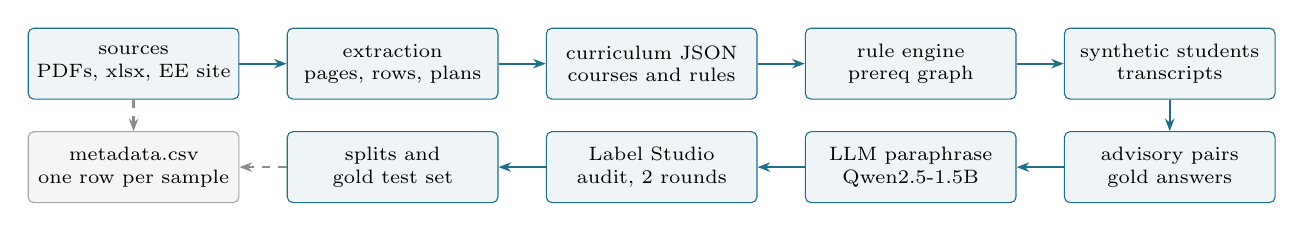
\begin{tikzpicture}[node distance=4mm and 6mm, every node/.style={font=\scriptsize}, box/.default=25mm, soft/.default=25mm]
\node[box] (src) {sources\\PDFs, xlsx, EE site};
\node[box, right=of src] (ext) {extraction\\pages, rows, plans};
\node[box, right=of ext] (cat) {curriculum JSON\\courses and rules};
\node[box, right=of cat] (eng) {rule engine\\prereq graph};
\node[box, right=of eng] (stu) {synthetic students\\transcripts};
\node[box, below=of stu] (pair) {advisory pairs\\gold answers};
\node[box, left=of pair] (para) {LLM paraphrase\\Qwen2.5-1.5B};
\node[box, left=of para] (ls) {Label Studio\\audit, 2 rounds};
\node[box, left=of ls] (gold) {splits and\\gold test set};
\node[soft, left=of gold] (meta) {metadata.csv\\one row per sample};
\draw[arr] (src) -- (ext); \draw[arr] (ext) -- (cat); \draw[arr] (cat) -- (eng); \draw[arr] (eng) -- (stu);
\draw[arr] (stu) -- (pair); \draw[arr] (pair) -- (para); \draw[arr] (para) -- (ls); \draw[arr] (ls) -- (gold);
\draw[arr, dashed, black!45] (gold) -- (meta);
\draw[arr, dashed, black!45] (src.south) -- (meta.north);
\end{tikzpicture}
\caption{Data flow from the sources to the gold set. Dashed: every layer also writes its rows to
\texttt{metadata.csv} [\ev{dataflow}, \ev{meta}].}\label{fig:flow}
\end{figure}

\section{Part B: Data validation}
\begin{keybox}
\kn{25}{checks: Pandera, networkx, rapidfuzz, rule engine [\ev{suite}]}\hfill
\kn{7 of 10}{raw-catalog checks fail [\ev{raw}]}\hfill
\kn{24 + 1}{processed: pass + one warning [\ev{proc}]}\hfill
\kn{15 of 15}{injected faults caught [\ev{faults}]}\hfill
\kn{2}{gold bugs found by people [\ev{fixai}, \ev{fixug}]}
\end{keybox}

\subsection{Validation suite.}
25 checks run on the raw catalog, the processed data and a corrupted copy, using Pandera schemas, networkx graph
checks, rapidfuzz title matching and the rule engine itself [\ev{suite}]. They cover the Project 4 checks:
prerequisites exist (V11), no cycles (V12), credit totals (V13), no duplicate codes (V06), transcripts pass the
engine (V17 to V20) and no student or template in both train and test (V25) [\ev{checkmap}].

\subsection{Before and after.}
On the raw catalog 7 of 10 applicable checks fail; on processed data 24 pass and V10 warns about two different
courses with near-identical titles, kept on purpose (Figure~\ref{fig:val}) [\ev{raw}, \ev{proc}].

\begin{figure}[h]
\centering
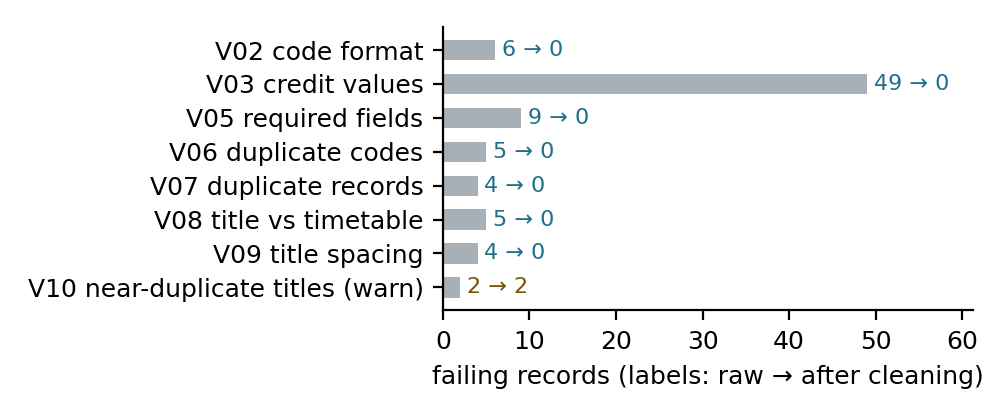
\includegraphics[width=4.2in]{fig_validation.png}
\caption{Failing records per check before and after cleaning [\ev{beforeafter}]. Full table:
Table~\ref{tab:ba}.}\label{fig:val}
\end{figure}

\subsection{Corrupted data.}
A DVC stage injects 15 faults with seed 209, among them a prerequisite cycle, an unknown prerequisite, total
credits changed from 82 to 80, a below-600 cap breach and train/test leakage; all 15 are caught [\ev{faults},
\ev{seedcorr}, \ev{fault82}]. One planned fault, a per-semester credit cap, was not injected because no source
states a cap [\ev{notinj}].

\subsection{What human review added.}
While labelling the first item, hem436 saw ``Other baskets (): 0 credits earned'' for an MTech-AI student: the
engine read other baskets from the student's own one-stream programme. The fix follows the CSE structure and changed
100 of 600 gold answers, all MTech-AI [\ev{fixai}]. Later hem436 noticed answers telling M.Tech students they lacked
IITGN UG courses; D5 removed these warnings and changed 53 gold answers and 0 query texts [\ev{fixug}]. Both have
regression tests and came before any finished annotation. The AI fix would have changed 12 of the 180 students, so
generation keeps the old basket view while gold answers use the fixed rule [\ev{twelve}, \ev{ownbaskets}].

\section{Part C: Labelling and agreement}
\begin{keybox}
\kn{2 $\times$ 40}{items, both annotators [\ev{design}]}\hfill
\kn{0.38}{decision kappa in round 2, up from 0.23 [\ev{kappa}]}\hfill
\kn{0.35}{category kappa in round 2, up from 0.17 [\ev{kappa}]}\hfill
\kn{55 / 21 / 4}{accept / edit / reject [\ev{outcome}]}\hfill
\kn{76}{gold test items [\ev{gold}]}
\end{keybox}

\subsection{Guidelines.}
Round 1 used guidelines v1. After it we analysed every disagreement and wrote v2, which adds seven rules, each tied
to a round-1 item: state every gold fact, any contradicted number is a wrong fact, a clear edit-or-reject threshold,
query checks, two-problem items, gold is the truth, formatting is not an error (Appendix~\ref{app:c})
[\ev{v2rules}].

\subsection{Independent annotation.}
A1 (hem436) and A2 (myankb08) labelled the same items in Label Studio 1.23.2, separately, in two disjoint rounds of
40 drawn from the test split with seed 208 [\ev{design}, \ev{seedann}, \ev{ls}]. Each item shows the student, the
template query, the paraphrase, the gold answer and the rewritten justification. Labelling test items is how the gold
test set is built: the rounds only audit and correct the text, and no model is trained, tuned or selected on any
test item. Figure~\ref{fig:lab} shows the workflow.

\begin{figure}[h]
\centering
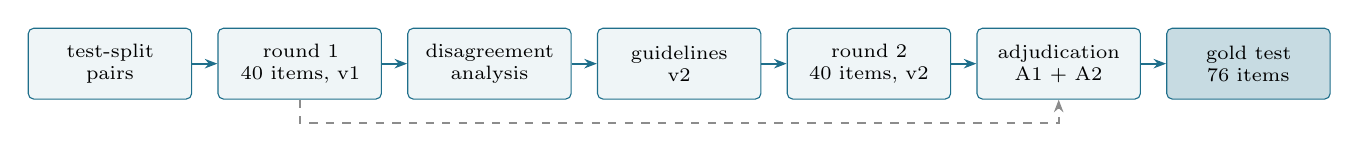
\begin{tikzpicture}[node distance=3.2mm, every node/.style={font=\scriptsize}]
\node[box] (p) {test-split\\pairs};
\node[box, right=of p] (r1) {round 1\\40 items, v1};
\node[box, right=of r1] (da) {disagreement\\analysis};
\node[box, right=of da] (v2) {guidelines\\v2};
\node[box, right=of v2] (r2) {round 2\\40 items, v2};
\node[box, right=of r2] (adj) {adjudication\\A1 + A2};
\node[box, right=of adj, fill=accent!25] (g) {gold test\\76 items};
\foreach \a/\b in {p/r1, r1/da, da/v2, v2/r2, r2/adj, adj/g} \draw[arr] (\a) -- (\b);
\draw[arr, dashed, black!45] (r1.south) -- ++(0,-3mm) -| (adj.south);
\end{tikzpicture}
\vspace{2pt}
\caption{Labelling workflow. Both rounds feed adjudication (dashed: round 1 disagreements) [\ev{design},
\ev{adjlog}, \ev{gold}].}\label{fig:lab}
\end{figure}

\subsection{Label order.}
Three levels in a fixed order: decision (accept, edit, reject), one error category, then the edit text
(Appendix~\ref{app:c}) [\ev{labelorder}]. Deciding first keeps the category list from steering the decision, and the
edit comes last, once the problem is named.

\subsection{Agreement.}
Decision kappa went from 0.227 [0.000, 0.469] to 0.377 [0.094, 0.630], and category kappa from 0.171
[0.007, 0.353] to 0.350 [0.064, 0.620], with 2000 bootstrap resamples [\ev{kappa}, \ev{nboot}]. Raw agreement went
from 65.0\% to 77.5\% on decision and from 62.5\% to 75.0\% on category; disagreements fell from 17 to 12
[\ev{rawagr}, \ev{ndis}]. The CIs overlap and the rounds use different items, so the gain is in the expected
direction but not conclusive. Round 1 was about strictness: A2 accepted 34 of 40 items and A1 24, and in 11 of the
17 disagreements A1 flagged an item that A2 accepted [\ev{accepts}, \ev{flagged}]. Causes: vague ``almost there''
justifications, wrong numbers in fluent text, the edit-or-reject threshold, and fixing correct gold from memory. In
round 2 the main split left was wrong numbers in fluent text, and the paraphraser kept turning ``coursework track''
into ``workshop track''.

\begin{figure}[h]
\centering
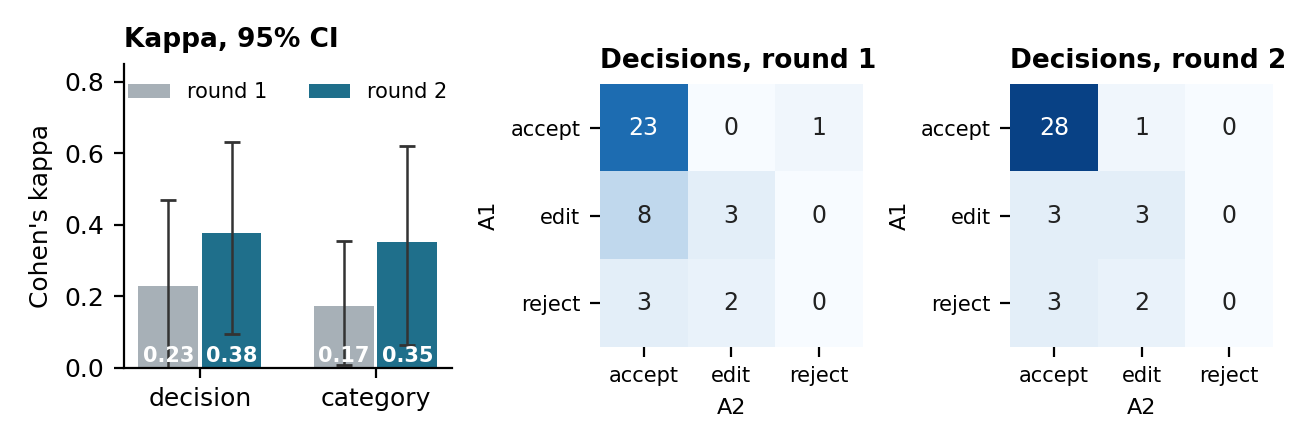
\includegraphics[width=0.9\textwidth]{fig_kappa.png}
\caption{Left: Cohen's kappa with bootstrap 95\% CI [\ev{kappa}]. Middle and right: decision confusion, A1 rows and
A2 columns, round 1 and round 2 [\ev{confusion}].}\label{fig:conf}
\end{figure}

\subsection{Gold test set.}
50 items agreed fully; the other 30 (17 in round 1, 13 in round 2) are the 29 disagreements plus one item where both
chose edit with different texts [\ev{adjlog}]. The assistant drafted a proposal for each of the 30 with a one-line
reason [\ev{proposals}]; A1 and A2 reviewed the 29 disagreements together, approving 28 and overriding 1
[\ev{decisions}], and A1 decided the extra item [\ev{extra}]. None stayed unresolved [\ev{unresolved}]. The gold test
set is the 76 accepted or edited items (27 eligibility, 27 elective recommendation, 22 remaining requirements),
frozen with sha256 \texttt{cd2e08dc\dots} [\ev{goldintent}, \ev{sha}].

\subsection{Real queries.}
\nforms{} consenting responses were imported, \nformsexcluded{} excluded; \nformsvone{} came from form v1 and
\nformsvtwo{} from v2, which added three example questions after respondents were unsure what to ask [\ev{forms},
\ev{formsexcl}, \ev{formver}]. \nformsproxy{} questions were asked in person by classmates and entered by hem436
after rewording with ChatGPT; the \nformsself{} self-submitted rows keep the students' own words [\ev{prov}]. They are
informal (``sem 3 of m.tech EE,SPML stream'') and often fall outside the three intents, so they form the
out-of-distribution shifted split. By kind: \nformsremaining{} remaining requirements, \nformselective{} elective
advice, \nformseligibility{} eligibility, \nformsother{} other [\ev{formkind}].

\section{Part D: Augmentation and active learning}
\begin{keybox}
\kn{1526}{of 1610 augmented pairs kept [\ev{children}]}\hfill
\kn{36 of 120}{LLM paraphrases kept [\ev{inv}]}\hfill
\kn{232 of 336}{base-model answers wrong [\ev{alpool}]}\hfill
\kn{0.43}{failures found by top-k at budget 100; random 0.30 [\ev{al}]}
\end{keybox}

\subsection{Augmentation.}
Typo and transcript children must leave the gold answer unchanged; transcript-length children must get the correctly
recomputed answer. LLM paraphrase children must also keep every fact the question states (programme, stream, track,
semesters completed, number of electives, term) and must not turn the question back on the student [\ev{slots}].
Most LLM paraphrases fail this: the track is lost in 47 failures (26 of them track alone), semesters completed in 35,
stream in 21, and 10 turn the question to the student [\ev{slotcounts}], the same ``workshop track'' errors the
annotators caught. The typo and transcript checks pass at 1.0 by construction, since those transforms never touch
the facts the engine reads.

\begin{figure}[h]
\centering
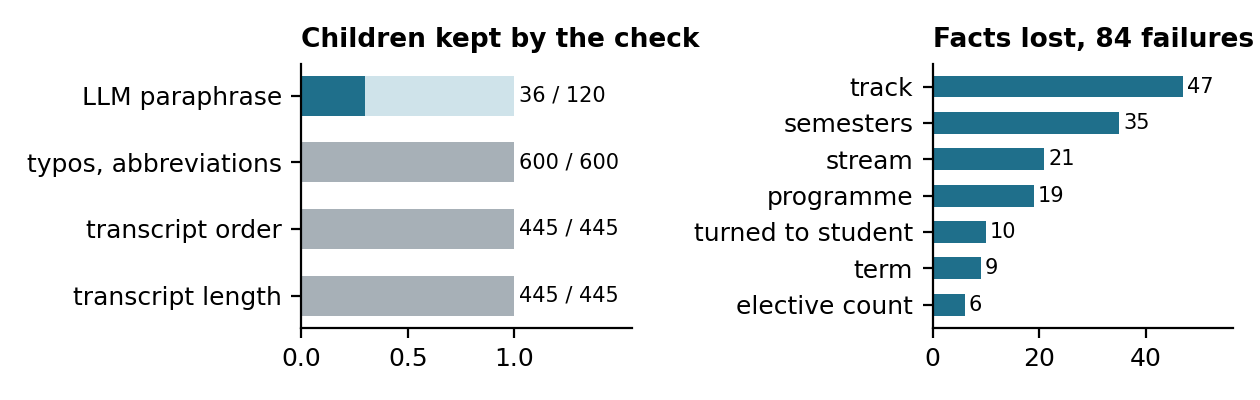
\includegraphics[width=0.92\textwidth]{fig_augment.png}
\caption{Left: share of children each check keeps [\ev{inv}]. Right: facts lost by the failed LLM paraphrases (one
can lose several) [\ev{slotcounts}]. Full table: Table~\ref{tab:aug}.}\label{fig:aug}
\end{figure}

\subsection{Active learning.}
The base model (same Qwen, greedy) answered the 336 train pairs; 232 answers are wrong: wrong remaining 94,
ineligible recommendation 64, wrong eligibility 56, invalid JSON 18, hallucinated code 2 [\ev{alpool}, \ev{altypes}].
Random is the mean of 5 seeds [\ev{seedal}]. The score and the failure test are the same comparison, so every top-k
pick is a failure (precision 1 by construction); the informative part is which failures each strategy reaches
[\ev{alread}]. Plain top-k takes every pick from one intent and covers 0.60 of the failure types; the
intent-stratified variant, added after the first run, keeps most of the gain (0.38 at budget 100) and covers all
failure types and intents [\ev{al}, \ev{strat}]. This is a label-efficiency comparison, not a learning curve.

\begin{figure}[h]
\centering
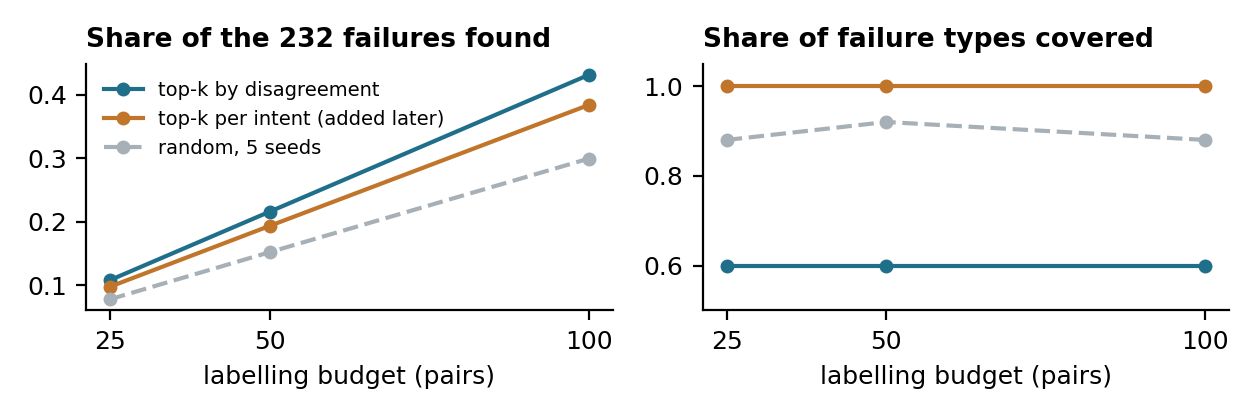
\includegraphics[width=0.85\textwidth]{fig_al.png}
\caption{Left: share of the 232 base-model failures each strategy finds; right: share of failure types it reaches
[\ev{al}]. Full table: Table~\ref{tab:al}.}\label{fig:al}
\end{figure}

\section{Part E: Versioning and splits}
\begin{keybox}
\kn{26}{DVC pipeline stages [\ev{stages}]}\hfill
\kn{0}{students shared between splits [\ev{overlap}]}\hfill
\kn{7 of 22}{templates used only in test [\ev{templates}]}\hfill
\kn{24}{ICDT students held out [\ev{splittab}]}\hfill
\kn{\nforms}{real questions in the shifted split [\ev{forms}]}
\end{keybox}

\subsection{Versioning.}
Human and raw inputs (sources, plans, form CSV, LLM cache, labelling files) are added with \texttt{dvc add};
everything else comes from the 26 stages, with EE fetching frozen [\ev{dvcadd}, \ev{stages}]. The remote is a local
folder next to the repo [\ev{remote}]. \texttt{dvc.lock} pins every output, and a full offline \texttt{dvc repro}
reproduced courses, rules, students, pairs, paraphrases, splits, labels, the gold set and base-model answers byte for
byte; only the run-time column of the metadata file differs [\ev{lock}, \ev{repro}].

\subsection{Splits.}
Students are assigned first, per programme (seed 207; 0.65 / 0.15 / 0.20), and each pair is then written with a
template allowed in its split [\ev{splitseed}]; one template per family is test-only. All MTech-ICDT students form a
programme holdout (the smallest programme and the only one without streams), and the real form questions form the
shifted split. Augmented pairs inherit their parent's split. All overlap checks are zero and no pair was dropped
[\ev{overlap}]; eligibility is balanced in every split (17 eligible and 17 not in test) [\ev{splittab}].

\begin{figure}[h]
\centering
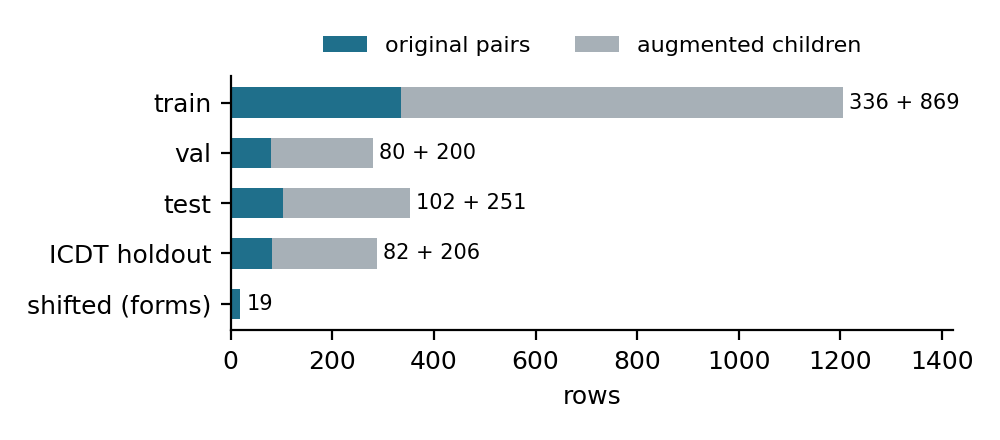
\includegraphics[width=4.4in]{fig_splits.png}
\caption{Rows per split: original pairs plus augmented children [\ev{splittab}, \ev{forms}]. Full table:
Table~\ref{tab:split}.}\label{fig:split}
\end{figure}

\subsection{Final tag.}
The tag \texttt{a1-final} is \freezestatus{} [\ev{tag}].

\section{Part F: Report and reproducibility}
\begin{keybox}
\kn{252}{tests pass [\ev{pytest}]}\hfill
\kn{8}{seeds in params.yaml [\ev{seeds}]}\hfill
\kn{3}{LLM backends, recorded per row [\ev{backends}]}\hfill
\kn{3.10.12}{Python; DVC 3.67.1 [\ev{env}]}
\end{keybox}

\subsection{Dataset card.}
DATASET\_CARD.md gives the sources, sizes (104 courses, 180 students, 600 pairs plus augmented children), balance
(200 pairs per intent; 100 eligible and 100 not) and known biases: synthetic students, no enforceable prerequisites,
credit defaults, a partial ICDT list, one known timetable term and a small real-query set [\ev{card}, \ev{pairs},
\ev{elig}].

\subsection{Data reproducibility.}
ENVIRONMENT.md records the laptop (Ubuntu 22.04.5, Ryzen 5 2500U, CPU only), Python, DVC, Label Studio, the model
digest and the Kaggle GPU (Tesla T4, CUDA 12.8, torch 2.11.0+cu128, transformers 5.16.1) [\ev{env}, \ev{gpu}]. The
pipeline prompt README lists model, versions and backends per prompt [\ev{promptreadme}]; all eight seeds live in
\texttt{params.yaml} [\ev{seeds}]. LLM answers are replayed from the DVC-tracked cache, so a rerun gives the same
text without a GPU.

\subsection{Label reproducibility.}
LABELLING\_PROTOCOL.md records who labelled what, tool versions, config and guidelines per round, label order, item
order and seed, what annotators saw, the adjudication process and a timeline matched to the exports, which are never
edited [\ev{protocol}].

\subsection{Repository and README.}
The README maps each Part to its code and outputs and rebuilds everything with four commands [\ev{readme}]:
\begin{tcolorbox}[colback=black!4,colframe=black!4,boxrule=0pt,arc=2pt,left=6pt,top=2pt,bottom=2pt,before skip=3pt,after skip=3pt]
\small\ttfamily\setstretch{1.0}
python3.10 -m venv .venv \&\& .venv/bin/pip install -r requirements.txt\\
.venv/bin/dvc pull \&\& .venv/bin/dvc repro \&\& .venv/bin/pytest -q
\end{tcolorbox}

\section{Limitations}
\begin{itemize}
\item Students are synthetic and valid by construction; no source states an enforceable PG prerequisite, so
  eligibility mostly tests offering and already-taken rules. Kappa rests on 40 items per round, so the CIs are wide.
\item LLM backends are mixed: Ollama 0.1.38 could not load the qwen2 tokenizer, so the same weights ran on llama.cpp,
  and part of the paraphrases ran on a Kaggle T4. Each row records its backend; outputs differ across backends
  [\ev{backends}, \ev{parabackend}].
\item Form examples were added mid-collection, which may pull later wording toward them. We have \nforms{} real
  questions, below the target of 30; \nformsproxy{} were reworded with ChatGPT, so only \nformsself{} keep the
  students' own words [\ev{target}, \ev{prov}].
\item The EE site marks the ICDT list ``to be updated soon'', so ICDT answers rest on a partial list [\ev{icdt}].
\end{itemize}

\section{Contribution table}
\begin{center}\small\setstretch{1.0}
\begin{tabular}{@{}>{\raggedright\arraybackslash}p{4.3cm}p{1.3cm}>{\raggedright\arraybackslash}p{10.7cm}@{}}
\toprule
member & commits & work \\
\midrule
Myank Singh Beniwal (25210087; myankb08) & \ncommitsM & First data-loading commit; annotator A2 in both rounds (exports committed from his
own account); joint adjudication with A1 (all 29 reviewed decisions are A1+A2). The docs record form distribution by
hem436 only [\ev{commits}, \ev{a2exports}, \ev{formshare}]. \\
Shekhar Mohanty Hement (25210122; hem436) & \ncommitsH & Everything else: scope decisions, pipeline and rule engine (built with Claude
Code), sources, form creation and sharing, annotator A1, joint adjudication, DVC, documentation and this report. \\
\bottomrule
\end{tabular}
\end{center}
\label{endofbody}

\clearpage
\appendix
\section{Evidence index}\label{app:a}
Every number in the body, with the file that backs it (paths from the repo root) and the field or row.
{\small\setstretch{1.0}
\begin{longtable}{@{}p{0.9cm}p{5.6cm}p{9.7cm}@{}}
\toprule
id & what & file and field \\
\midrule
\endhead
\evgroup{1 Introduction}
\evrow{scope}{4 programmes, thesis and coursework tracks}{\f{docs/DECISIONS.md}, rows D1, D2, D3}
\evrow{courses}{104 courses}{\f{data/processed/courses.json}, list length; \f{supporting_files/B_engine/prereq_graph_report.json} \f{nodes}}
\evrow{rules}{77 rules; 20 EE (\f{ee.*}); 1 not stated (max credits per semester)}{\f{data/processed/rules.json}, \f{rules} keys, prefix \f{ee.}, \f{not_stated: true}}
\evrow{students}{180 students; CSE 64, EE 51, AI 41, ICDT 24; 92 thesis, 88 coursework; 1422 entries; 0 violations}{\f{supporting_files/B_engine/transcripts_summary.json}, \f{n_students}, \f{programmes}, \f{tracks}, \f{transcript_entries}, \f{violations}}
\evrow{pairs}{600 pairs, 200 per intent}{\f{supporting_files/B_engine/queries_summary.json}, \f{n_pairs}, \f{per_intent}}
\evrow{children}{1526 children kept of 1610}{\f{supporting_files/E_splits/split_summary.json} \f{n_children_in} (sum of \f{child_rows_per_split}); \f{supporting_files/D_augmentation/verify_report.json} \f{children_in}}
\evrow{audited}{80 audit items (40 per round)}{\f{data/labels/audited.jsonl}, row count by \f{round}}
\evrow{gold}{76 gold test items}{\f{supporting_files/E_splits/gold_summary.json}, \f{n_gold}}
\evrow{forms}{\nforms{} real form questions}{\f{supporting_files/C_labelling/forms_import_log.json} \f{rows_kept}; \f{supporting_files/E_splits/shifted_summary.json} \f{n_rows}}
\evgroup{2 Part A: Collection and instrumentation}
\evrow{sources}{8 advisories, CSE structure, timetable, 4 EE pages, each with sha256}{\f{data/raw/sources/source_metadata.json} \f{sources[].sha256}; \f{data/metadata.csv} rows with \f{artifact} under \f{data/raw/sources/}}
\evrow{meta}{\nmeta{} metadata rows (\nmetaraw{} raw, \nmetaproc{} processed)}{\f{data/metadata.csv}, row count and \f{layer} counts}
\evrow{metakinds}{180 / 600 / 1526 / \nforms{} / 76 rows for students, pairs, children, forms, rules (76 of 77)}{\f{data/metadata.csv}, \f{sample_id} prefixes \f{student}, \f{pair}, \f{aug}, \f{form}, \f{rule}}
\evrow{plancs}{50 CS/ES codes: 15 downloaded, 12 login, 23 no link}{\f{supporting_files/A_collection/course_plan_fetch_log.csv}, last \f{outcome} per \f{code}}
\evrow{planee}{25 EE codes: 7, 4, 14}{\f{supporting_files/A_collection/ee_course_plan_fetch_log.csv}, same}
\evrow{planfiles}{22 plan files (15 + 7)}{\f{data/raw/course_plans/}, file count}
\evrow{rawcat}{136 raw catalog records}{\f{data/metadata.csv} rows with \f{artifact} = \f{data/raw/catalog_raw.json}; \f{supporting_files/A_collection/collection_log.md} section 7}
\evrow{coursecat}{67 / 15 / 6 / 2 / 6 / 8 courses by category}{\f{data/processed/courses.json}, \f{category}}
\evrow{changes}{78 cleaning changes}{\f{supporting_files/A_collection/cleaning_changes.csv}, data rows}
\evrow{prereq}{103 none stated, 1 manual; 0 enforceable}{\f{data/processed/courses.json}, \f{prereq_source} and empty \f{prerequisites}}
\evrow{cs613}{CS 613 manual decision}{\f{data/raw/prereq_manual.csv}, \f{decided_by}}
\evrow{recbg}{3 courses with recommended background}{\f{data/processed/courses.json}, non-empty \f{recommended_background}}
\evrow{graph}{104 nodes, 9 recommended edges, 0 missing, 0 cycles}{\f{supporting_files/B_engine/prereq_graph_report.json}, \f{nodes}, \f{edges_by_type}, \f{missing_prereq_codes}, \f{cycles}}
\evrow{d4d5}{decisions D4, D5}{\f{docs/DECISIONS.md}, rows D4, D5}
\evrow{seedtr}{seed 203}{\f{params.yaml}, \f{seeds.transcripts}}
\evgroup{3 Part B: Data validation}
\evrow{suite}{25 checks, V01 to V25}{\f{supporting_files/B_validation/processed/results.csv}, 25 rows; libraries in \f{requirements.txt}}
\evrow{raw}{raw: 10 checks, 7 fail, 2 pass, 1 warn}{\f{supporting_files/B_validation/raw/results.csv}, \f{status}}
\evrow{proc}{processed: 24 pass, 1 warn (V10, 2)}{\f{supporting_files/B_validation/processed/results.csv}, \f{status}, \f{n_failures}}
\evrow{beforeafter}{Figure~\ref{fig:val} and Table~\ref{tab:ba} values}{\f{supporting_files/B_validation/before_after.md}, table rows}
\evrow{faults}{15 of 15 faults caught}{\f{supporting_files/B_validation/corrupted/faults_caught.json}, \f{caught}}
\evrow{fault82}{total credits 82 to 80}{same, F05 \f{description}}
\evrow{notinj}{1 fault not injected}{\f{data/interim/corrupted/faults.json} (output of DVC stage \f{validate_corrupted}), \f{not_injected}}
\evrow{seedcorr}{seed 209}{\f{params.yaml}, \f{seeds.validation_corruption}}
\evrow{fixai}{100 of 600 gold answers changed (AI fix)}{\f{supporting_files/B_engine/gold_fix_mtech_ai_baskets.md}, ``Effect''}
\evrow{fixug}{53 gold answers, 0 query texts changed (D5)}{\f{supporting_files/B_engine/gold_fix_ug_background.md}, ``Effect''}
\evrow{twelve}{12 of 180 students the AI fix would change}{\f{supporting_files/B_engine/gold_fix_mtech_ai_baskets.md}, last section}
\evrow{ownbaskets}{old basket view kept for generation}{\f{src/engine/rule_engine.py}, \f{role_of} docstring}
\evgroup{4 Part C: Labelling and agreement}
\evrow{design}{40 items per round, 2 rounds}{\f{supporting_files/C_labelling/round1/agreement_summary.json} and \f{round2/}, \f{n_items_compared}}
\evrow{seedann}{seed 208}{\f{params.yaml}, \f{seeds.annotation_order}}
\evrow{ls}{Label Studio 1.23.2}{\f{ENVIRONMENT.md}, Python and tools table}
\evrow{v2rules}{seven v2 rules (R1 to R7)}{\f{supporting_files/C_labelling/round1/disagreement_analysis.md}, ``Changes for guidelines v2''}
\evrow{kappa}{kappa 0.227, 0.171, 0.377, 0.350 and their 95\% CIs}{\f{supporting_files/C_labelling/kappa_ci.json}, \f{round*_decision}, \f{round*_error_category}}
\evrow{nboot}{2000 resamples}{same, \f{n_boot}}
\evrow{confusion}{confusion matrices}{\f{supporting_files/C_labelling/round1/confusion_decision.csv} and \f{round2/}}
\evrow{rawagr}{raw agreement 65.0 / 62.5 and 77.5 / 75.0\%}{\f{supporting_files/C_labelling/round1/agreement_summary.json} and \f{round2/}, \f{percent_agreement}}
\evrow{ndis}{17 and 12 disagreements}{same, \f{n_disagreements}}
\evrow{accepts}{A2 accepted 34, A1 24 (round 1)}{\f{supporting_files/C_labelling/round1/agreement_summary.json}, \f{label_counts}}
\evrow{flagged}{11 of 17: A1 flagged, A2 accepted}{\f{supporting_files/C_labelling/round1/disagreement_analysis.md}, ``The main pattern''}
\evrow{adjlog}{50 agreed; 17 + 13 adjudicated}{\f{supporting_files/C_labelling/adjudication_log.json}, \f{agreed}, \f{adjudicated}}
\evrow{proposals}{30 proposals (29 + R2-Q0196)}{\f{supporting_files/C_labelling/adjudication_proposals.json}, keys other than \f{_about}}
\evrow{decisions}{28 approved, 1 overridden, all A1+A2}{\f{supporting_files/C_labelling/adjudication_decisions_export.json}, \f{choice}, \f{decided_by}}
\evrow{extra}{extra item decided by A1}{\f{data/labels/audited.jsonl}, \f{decided_by} of R2-Q0196}
\evrow{unresolved}{0 unresolved}{\f{supporting_files/C_labelling/adjudication_log.json}, \f{unresolved_items}}
\evrow{outcome}{55 accept, 21 edit, 4 reject}{\f{data/labels/audited.jsonl}, \f{final_decision}}
\evrow{goldintent}{gold by intent 27 / 27 / 22}{\f{supporting_files/E_splits/gold_summary.json}, \f{by_intent}}
\evrow{sha}{sha256 \f{cd2e08dcb56f5716b06981e096c3c93fd417abab1989b5d22d45befeafbc383f}}{\f{data/gold/GOLD_SHA256.txt}, line 1}
\evrow{formsexcl}{\nformsexcluded{} excluded}{\f{supporting_files/C_labelling/forms_import_log.json}, \f{rows_excluded}}
\evrow{formver}{\nformsvone{} v1, \nformsvtwo{} v2}{\f{supporting_files/E_splits/shifted_summary.json}, \f{by_form_version}}
\evrow{prov}{\nformsself{} self-submitted, \nformsproxy{} entered after ChatGPT rewording}{same, \f{by_provenance}; \f{supporting_files/C_labelling/forms_log.md}}
\evrow{formkind}{\nformsremaining{} / \nformselective{} / \nformseligibility{} / \nformsother{} by kind}{same, \f{by_question_kind}}
\evgroup{5 Part D: Augmentation and active learning}
\evrow{inv}{36 of 120 paraphrases; Figure~\ref{fig:aug} left and Table~\ref{tab:aug}}{\f{supporting_files/D_augmentation/invariance.csv}, all rows}
\evrow{slots}{facts the paraphrase check compares}{\f{src/augment/verify.py}, \f{slot_issues}}
\evrow{slotcounts}{track 47 (26 alone), semesters 35, stream 21, turned to student 10}{\f{supporting_files/D_augmentation/invariance.csv}, \f{fail_reasons}, counts summed over every reason that names the slot}
\evrow{alpool}{336 pool pairs, 232 failures}{\f{supporting_files/D_active_learning/scores_summary.json}, \f{n}, \f{failed}}
\evrow{altypes}{94 / 64 / 56 / 18 / 2 by failure type}{same, \f{failure_types}}
\evrow{al}{0.43, 0.38, 0.30 at budget 100; 0.60 types; Figure~\ref{fig:al} and Table~\ref{tab:al}}{\f{supporting_files/D_active_learning/label_efficiency.csv}, \f{failures_captured}, \f{failure_types_covered}, \f{intents_covered}}
\evrow{seedal}{5 random seeds}{\f{params.yaml}, \f{seeds.active_learning}}
\evrow{alread}{precision 1 by construction; not a learning curve}{\f{supporting_files/D_active_learning/summary.md}, ``Reading the first column''}
\evrow{strat}{stratified variant added later}{same, paragraph after it}
\evgroup{6 Part E: Versioning and splits}
\evrow{stages}{26 stages, EE fetch frozen}{\f{dvc.yaml}, \f{stages}, \f{fetch_ee_pages: frozen}}
\evrow{dvcadd}{inputs added with dvc add}{\f{data/raw/*.dvc}, \f{data/raw/forms/responses_raw.csv.dvc}, \f{data/interim/llm_cache.jsonl.dvc}, \f{data/labels/round*/*.dvc}}
\evrow{remote}{local remote \f{../dvc_remote}}{\f{.dvc/config} \f{remote "localremote"}; \f{README.md}}
\evrow{lock}{every output pinned}{\f{dvc.lock}, stage \f{outs} hashes}
\evrow{repro}{byte-for-byte rerun}{\f{supporting_files/F_reproducibility/repro_check.txt}, \f{sha256sum -c} lines, \f{dvc status}}
\evrow{tag}{tag a1-final}{\f{HANDOFF_A2.md}, first paragraph}
\evrow{splitseed}{seed 207; 0.65 / 0.15 / 0.20}{\f{supporting_files/E_splits/split_summary.json}, \f{seed}, \f{fractions}}
\evrow{templates}{7 of 22 templates test-only}{same, \f{held_out_templates}; \f{supporting_files/B_engine/queries_summary.json} \f{per_template}}
\evrow{overlap}{all overlaps 0, 0 dropped}{\f{supporting_files/E_splits/split_summary.json}, \f{overlap_checks}, \f{all_overlaps_zero}, \f{n_dropped_pairs}}
\evrow{splittab}{Figure~\ref{fig:split} and Table~\ref{tab:split} values; 24 ICDT students; 17 / 17 in test}{same, \f{student_assignment}, \f{original_rows_per_split}, \f{child_rows_per_split}, \f{rows_per_split}, \f{eligibility_by_split}, \f{original_rows_by_programme}}
\evgroup{7 to 9 Part F, limitations, contribution table}
\evrow{pytest}{252 tests pass}{\f{supporting_files/F_reproducibility/pytest.txt}, last line}
\evrow{seeds}{8 seeds}{\f{params.yaml}, \f{seeds}}
\evrow{env}{Ubuntu 22.04.5, Ryzen 5 2500U, Python 3.10.12, DVC 3.67.1}{\f{ENVIRONMENT.md}, Machine and Python and tools tables}
\evrow{gpu}{Tesla T4, CUDA 12.8, torch 2.11.0+cu128, transformers 5.16.1}{\f{ENVIRONMENT.md}, GPU row}
\evrow{promptreadme}{model, versions, backends per prompt}{\f{prompts/pipeline/README.md}, Model and Prompts}
\evrow{backends}{3 backends; Ollama 0.1.38, llama.cpp, Kaggle T4}{\f{supporting_files/D_augmentation/llm_backend.md}, sections 1, 2, 4}
\evrow{parabackend}{backend per row}{\f{data/processed/queries_para.jsonl}, \f{para_backend}}
\evrow{target}{target of 30 real queries}{assignment brief (not in the zip), Section 8, Project 4: ``at least 30 real queries''}
\evrow{icdt}{ICDT list ``to be updated soon''}{\f{supporting_files/A_collection/collection_log.md} section 7; \f{DATASET_CARD.md}}
\evrow{commits}{\ncommitsH{} / \ncommitsM{} commits}{git history: \texttt{git log -{}-format=\%an | sort | uniq -c}}
\evrow{a2exports}{A2 exports committed by myankb08}{\texttt{git log -{}-author=myankb08} (both \f{export_A2.json} commits); \f{LABELLING_PROTOCOL.md} section 9}
\evrow{formshare}{form shared by hem436}{\f{supporting_files/C_labelling/forms_log.md}, row 2}
\evrow{sessions}{17 requests to the assistant}{\f{prompts/assistant/user_requests.md}, table rows}
\evgroup{Added with the section structure (2.1 to 7.4)}
\evrow{metafields}{metadata fields: source, timestamp, collector, tool, tool version, content hash}{\f{data/metadata.csv} header (\f{source_doc}, \f{source_page}, \f{collected_at_utc}, \f{collector}, \f{tool}, \f{tool_version}, \f{content_sha256}); \f{docs/DATA_CONTRACT.md} ``Metadata''}
\evrow{licence}{licences and use of institute documents and course plans}{\f{docs/CONSENT_AND_LICENSING.md}, ``Institute documents'', ``Course plans''}
\evrow{consent}{consent register, one row per response}{\f{data/consent_register.csv} (output of DVC stage \f{import_forms}), \f{consent_given}, \f{form_version}}
\evrow{dataflow}{data flow and stage order}{\f{docs/DATA_FLOW.md}; \f{dvc.yaml} \f{stages}}
\evrow{collog}{collection log}{\f{supporting_files/A_collection/collection_log.md}}
\evrow{checkmap}{Project 4 checks V06, V11, V12, V13, V17 to V20, V25}{\f{supporting_files/B_validation/processed/results.csv}, \f{check_id}, \f{description}}
\evrow{labelorder}{label order decision, category, edit}{\f{LABELLING_PROTOCOL.md} section 5; \f{labelstudio/config_v1.xml}}
\evrow{card}{dataset card: sources, sizes, balance, biases}{\f{DATASET_CARD.md}, sections Sources, Sizes, Splits and balance, Known biases and limits}
\evrow{elig}{100 eligible, 100 not eligible pairs}{\f{supporting_files/B_engine/queries_summary.json}, \f{eligibility_eligible}, \f{eligibility_not_eligible}}
\evrow{protocol}{labelling protocol contents}{\f{LABELLING_PROTOCOL.md}, sections 1 to 9}
\evrow{readme}{README part map and rebuild commands}{\f{README.md}, ``Rebuild the data'', ``Where each part lives''}
\bottomrule
\end{longtable}
}
\addtocounter{table}{-1}

\section{AI assistance}\label{app:b}
\textbf{What the assistant did.} Claude Code (model claude-opus-5-5) wrote most of the code through sub-agents whose
prompts are in \f{prompts/assistant/}: \f{agent_common_rules.md}, \f{agent_A_curriculum.md}, \f{agent_A2_ee_pages.md},
\f{agent_B_engine.md}, \f{agent_B2_engine_revision.md}, \f{agent_C_labelling.md}, \f{agent_D_validation.md},
\f{agent_E_llm_augment_al.md}, \f{agent_F_splits_dvc_docs.md}, \f{agent_F2_resplit.md}, \f{agent_G_report.md} and
\f{agent_G2_report_redesign.md} (this report). hem436's own requests
to the assistant are summarised, each with the files it changed, in \f{user_requests.md} [\ev{sessions}]. The assistant also drafted the 30 adjudication proposals (people made every final call),
built the labelling kit pages and the adjudication review page, and built and edited the Google Form in the browser
at the user's request.

\textbf{ChatGPT.} hem436 used ChatGPT to reword \nformsproxy{} questions that classmates asked in person before
entering them in the form (\f{prompts/assistant/chatgpt_form_rewording.md}; the prompt and the original wording were
not kept).

\textbf{Pipeline LLM.} Qwen2.5-1.5B-Instruct (Q4\_K\_M via llama.cpp, or fp16 via transformers on Kaggle) paraphrases
queries and justifications and gives base-model answers. Its prompts are files in \f{prompts/pipeline/}:
\f{paraphrase_query_v1.txt}, \f{paraphrase_justification_v1.txt}, \f{augment_paraphrase_v1.txt} and
\f{base_model_answer_v1.txt}. Model, digest and backend are stored with every output, and the README there lists
model, versions and backends per prompt and the Qwen default system prompt.

\textbf{What people did.} All labelling (A1 and A2, both rounds), every adjudication decision, the scope and
modelling decisions in \f{docs/DECISIONS.md}, both gold-bug findings, and form sharing and distribution.

\section{Guidelines v2 and label levels}\label{app:c}
\textbf{Label levels, in this order:} 1) decision: accept, edit or reject; 2) one error category, by priority:
hallucinated course, wrong fact or policy, meaning drift, incomplete justification, ambiguous query, fluency (or
none); 3) edit text, only for edit. The label set and the Label Studio config did not change between rounds.

\textbf{Changes from v1 to v2}, each tied to round-1 disagreements:
\begin{itemize}
\item R1: a justification must state the gold outcome and every number, course and open item; pure encouragement is
  an incomplete justification.
\item R2: any number or status that contradicts gold or is not in gold is a wrong fact, including vague text that
  implies a wrong status.
\item R3: edit when the fix touches at most two sentences or one query phrase, otherwise reject; a missing fact alone
  is never a reason to reject.
\item R4: added scope, ``available'' for ``remaining'', or a question turned back on the student is meaning drift.
\item R5: with two problems, pick the category by priority and fix both texts.
\item R6: gold is the truth; do not correct it from memory, write ``GOLD?'' instead.
\item R7: formatting and tone are not errors; edit or reject always needs a category other than none.
\end{itemize}

\clearpage
\section{Detailed tables}\label{app:d}
\begin{table}[!h]
\centering\small
\caption{Failing records before and after cleaning. Source: \f{supporting_files/B_validation/before_after.md}.}\label{tab:ba}
\begin{tabular}{@{}llrr@{}}
\toprule
check & what it tests & raw & after \\
\midrule
V02 & code format & 6 & 0 \\
V03 & credits are integers in range & 49 & 0 \\
V05 & required fields present & 9 & 0 \\
V06 & no duplicate codes & 5 & 0 \\
V07 & no exact duplicate records & 4 & 0 \\
V08 & title matches timetable & 5 & 0 \\
V09 & title spacing and punctuation & 4 & 0 \\
V10 & near-duplicate titles (warning) & 2 & 2 \\
\bottomrule
\end{tabular}
\end{table}

\begin{table}[!h]
\centering\small
\caption{Augmentation checks. Source: \f{supporting_files/D_augmentation/invariance.csv}.}\label{tab:aug}
\begin{tabular}{@{}llrrr@{}}
\toprule
augmentation & check & children & kept & rate \\
\midrule
LLM paraphrase & gold and stated facts unchanged & 120 & 36 & 0.30 \\
typos and abbreviations & gold unchanged & 600 & 600 & 1.00 \\
transcript order & gold unchanged & 445 & 445 & 1.00 \\
transcript length & gold recomputed correctly & 445 & 445 & 1.00 \\
\bottomrule
\end{tabular}
\end{table}

\begin{table}[!h]
\centering\small
\caption{Share of the 232 failures captured per budget, and coverage. Random is the mean of 5 seeds. Source:
\f{supporting_files/D_active_learning/label_efficiency.csv}.}\label{tab:al}
\begin{tabular}{@{}lrrrrr@{}}
\toprule
strategy & 25 & 50 & 100 & types & intents \\
\midrule
top-k by disagreement & 0.11 & 0.22 & 0.43 & 0.60 & 1 \\
stratified by intent (added later) & 0.10 & 0.19 & 0.38 & 1.00 & 3 \\
random & 0.08 & 0.15 & 0.30 & 0.88 to 0.92 & 3 \\
\bottomrule
\end{tabular}
\end{table}

\begin{table}[!h]
\centering\small
\caption{Split sizes. Students are those assigned; pairs per programme are CSE / AI / EE / ICDT. Source:
\f{supporting_files/E_splits/split_summary.json}; shifted row from \f{supporting_files/E_splits/shifted_summary.json}.}\label{tab:split}
\begin{tabular}{@{}lrrrrrr@{}}
\toprule
split & students & pairs & children & rows & eligible / not & by programme \\
\midrule
train & 101 & 336 & 869 & 1205 & 56 / 56 & 127 / 90 / 119 / 0 \\
val & 24 & 80 & 200 & 280 & 13 / 13 & 35 / 21 / 24 / 0 \\
test & 31 & 102 & 251 & 353 & 17 / 17 & 49 / 21 / 32 / 0 \\
ICDT holdout & 24 & 82 & 206 & 288 & 14 / 14 & 0 / 0 / 0 / 82 \\
shifted (forms) & n/a & \nforms{} & 0 & \nforms{} & n/a & n/a \\
\bottomrule
\end{tabular}
\end{table}

\end{document}
